\documentclass[a4paper,11pt]{article}
\usepackage{amsmath,amsthm,amsfonts,amssymb,amscd,amstext,vmargin,graphics,graphicx,tabularx,multicol} 
\usepackage[francais]{babel}
\usepackage[utf8]{inputenc}  
\usepackage[T1]{fontenc} 
\usepackage{pstricks-add,tikz,tkz-tab,variations}
\usepackage[autolanguage,np]{numprint} 

\setmarginsrb{1.5cm}{0.5cm}{1cm}{0.5cm}{0cm}{0cm}{0cm}{0cm} %Gauche, haut, droite, haut
\newcounter{numexo}
\newcommand{\exo}[1]{\stepcounter{numexo}\noindent{\bf Exercice~\thenumexo} : \marginpar{\hfill /#1}}
\reversemarginpar


\newcounter{enumtabi}
\newcounter{enumtaba}
\newcommand{\q}{\stepcounter{enumtabi} \theenumtabi.  }
\newcommand{\qa}{\stepcounter{enumtaba} (\alph{enumtaba}) }
\newcommand{\initq}{\setcounter{enumtabi}{0}}
\newcommand{\initqa}{\setcounter{enumtaba}{0}}

\newcommand{\be}{\begin{enumerate}}
\newcommand{\ee}{\end{enumerate}}
\newcommand{\bi}{\begin{itemize}}
\newcommand{\ei}{\end{itemize}}
\newcommand{\bp}{\begin{pspicture*}}
\newcommand{\ep}{\end{pspicture*}}
\newcommand{\bt}{\begin{tabular}}
\newcommand{\et}{\end{tabular}}
\renewcommand{\tabularxcolumn}[1]{>{\centering}m{#1}} %(colonne m{} centrée, au lieu de p par défault) 
\newcommand{\tnl}{\tabularnewline}

\newcommand{\bmul}[1]{\begin{multicols}{#1}}
\newcommand{\emul}{\end{multicols}}

\newcommand{\trait}{\noindent \rule{\linewidth}{0.2mm}}
\newcommand{\hs}[1]{\hspace{#1}}
\newcommand{\vs}[1]{\vspace{#1}}

\newcommand{\N}{\mathbb{N}}
\newcommand{\Z}{\mathbb{Z}}
\newcommand{\R}{\mathbb{R}}
\newcommand{\C}{\mathbb{C}}
\newcommand{\Dcal}{\mathcal{D}}
\newcommand{\Ccal}{\mathcal{C}}
\newcommand{\mc}{\mathcal}

\newcommand{\vect}[1]{\overrightarrow{#1}}
\newcommand{\ds}{\displaystyle}
\newcommand{\eq}{\quad \Leftrightarrow \quad}
\newcommand{\vecti}{\vec{\imath}}
\newcommand{\vectj}{\vec{\jmath}}
\newcommand{\Oij}{(O;\vec{\imath}, \vec{\jmath})}
\newcommand{\OIJ}{(O;I,J)}


\newcommand{\reponse}[1][1]{%
\multido{}{#1}{\makebox[\linewidth]{\rule[0pt]{0pt}{20pt}\dotfill}
}}

\newcommand{\titre}[5] 
% #1: titre #2: haut gauche #3: bas gauche #4: haut droite #5: bas droite
{
\noindent #2 \hfill #4 \\
#3 \hfill #5

\vspace{-1.6cm}

\begin{center}\rule{6cm}{0.5mm}\end{center}
\vspace{0.2cm}
\begin{center}{\large{\textbf{#1}}}\end{center}
\begin{center}\rule{6cm}{0.5mm}\end{center}
}



\begin{document}
\pagestyle{empty}
\titre{Interrogation: Volumes }{Nom :}{Prénom :}{Classe}{Date}


\exo{4} Calculer le volume des figures suivantes :\\

a) 
\includegraphics[scale=1.5]{vol1.eps}  \hspace*{1cm} b) 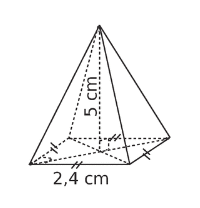
\includegraphics[scale=1.5]{vol2.eps} 

\bmul{2}
\color{red}
$V_{cone}=\dfrac{1}{3}\times \pi \times r^{2}\times h$\\

$V_{cone}=\dfrac{1}{3}\times \pi\times 3,3^{2}\times 5,6$\\

$V_{cone} \approx 63,86 cm^{3}$\\

\columnbreak


$V_{pyramide}=\dfrac{1}{3}\times A_{base} \times h$\\

$V_{pyramide}=\dfrac{1}{3}\times c^{2} \times h$\\

$V_{pyramide}=\dfrac{1}{3}\times 2,4^{2} \times 5$\\

$V_{pyramide}=9,6 cm^{3}$\\
\color{black}

\emul
\exo{2} Convertir les volumes suivants :

\bmul{2}

\qa 856 $mm^{3}$ = \textcolor{red}{0,856} $ cm^{3}$\\

\qa 1,356 $m^{3}$ = \textcolor{red}{1 356 000}  $ cm^{3}$


\columnbreak

\qa 95 000 $cm^{3}$ = \textcolor{red}{95}  $ L$\\

\qa 1 547 $L$ = \textcolor{red}{1,547}  $ m^{3}$

\emul

\vspace*{0.5cm}
\exo{4}  
\vspace*{0.5cm}
\color{red}
CORRECTION\\
\includegraphics[scale=1.5]{interrocorrection.eps} 




\end{document}
